\documentclass[10pt]{article}
\usepackage[letterpaper,margin=0.7in]{geometry}
\usepackage[T1]{fontenc}
\usepackage{lmodern}
\usepackage{microtype}
\usepackage{amsmath}
\usepackage{booktabs}
\usepackage{graphicx}
\usepackage{caption}
\captionsetup{font=small,skip=3pt}
\usepackage{xcolor}
\usepackage[hidelinks]{hyperref}
\usepackage{enumitem}
\setlist{nosep,leftmargin=1.2em}
\setlength{\parskip}{2pt}
\setlength{\parindent}{0pt}
\usepackage{titlesec}
\titlespacing*{\section}{0pt}{6pt}{2pt}
\titleformat{\section}{\normalsize\bfseries}{\thesection}{0.6em}{}

\newcommand{\repo}{https://github.com/JiaxiangCxx/ITCS8169_Assignment3}

\begin{document}

\begin{center}
{\large\bfseries One-Shot Scene Classification with Frozen Vision--Language Models\\and Test-Time Adaptation}\\[3pt]
ITCS 6169/8169 Computer Vision, Assignment 3 \quad$\cdot$\quad Jiaxiang Zhang
\end{center}

\vspace{-4pt}
\noindent\fcolorbox{black!40}{black!3}{\parbox{\dimexpr\linewidth-2\fboxsep-2\fboxrule}{
\textbf{Best test accuracy: 94.00\%} on the 400 labeled test images (main one-shot split, seed 0).
Averaged over 10 random one-shot splits: \textbf{94.50\,$\pm$\,0.56\%}.
Model: CLIP ViT-L/14-336 + SigLIP2 SO400M/16-512, both frozen, with test-time soft $k$-means.\\
\textbf{Code, trained model, inference script and instructions:} \url{\repo}.
\texttt{predict.py} reproduces the 94.00\% from raw images in about two minutes on one GPU.}}

\section{Task and the one-image rule}
The dataset has 16 scene classes (the 15-Scene categories plus \emph{Flower}) with small grayscale photos of about 250\,px.
There are 2400 training images (150 per class), 400 labeled test images (25 per class) and 400 unlabeled \texttt{test2} images.
We use \textbf{exactly one training image per class}, drawn at random with a fixed seed (\texttt{splits/oneshot\_seed0.json}).
The code never opens any other training image.
Seeds 1--9 draw different single images and are used only to measure how much the choice of image matters.
The text prompts use only the class names, and test labels are used only for scoring.

\section{One-shot recipe: frozen foundation models + test-time adaptation}
Sixteen images are far too few to train or fine-tune a network without over-fitting, but CLIP-style models already map scene photos and scene names into one embedding space.
We therefore keep the encoders frozen and only decide how to combine three sources of evidence: the class names, the single image, and the structure of the unlabeled test set.
All embeddings are L2-normalised.

\textbf{(a) Text classifier.} Each class gets 1--3 synonyms (e.g.\ \emph{OpenCountry} $\to$ ``open country'', ``an open countryside field'', ``a rural landscape'').
Each synonym fills 8 templates, three of which say ``black and white'' or ``grayscale'' because the whole dataset is grayscale.
The prompt embeddings are averaged into one text vector $t_k$ per class.

\textbf{(b) One-image prototype.} The training image of class $k$ is encoded as 34 views (center crop, horizontal flip, and 32 random resized crops with brightness/contrast jitter), and their mean is the prototype $p_k$.

\textbf{(c) Fusing across the modality gap.} Image--text and image--image similarities live on very different scales.
For CLIP-L, a test image's highest similarity to any class text vector averages 0.26, versus 0.85 to its nearest prototype (SigLIP2: 0.12 versus 0.78).
Adding raw scores would let the single image dominate, so each score matrix is standardised per test image over the 16 classes, $z(\cdot)$, and then summed: $s_{ik}=z(x_i^\top t_k)+z(x_i^\top p_k)$.

\textbf{(d) Test-time adaptation (transductive soft $k$-means).} A single image is a noisy estimate of a class, but the unlabeled test set shows where each class actually lies.
Starting from $\mu_k=p_k$, we iterate 20 times:
\[
q_{ik}=\operatorname{softmax}_k\!\big(\kappa\,[\,z(x_i^\top t_k)+z(x_i^\top \mu_k)\,]\big),\qquad
\mu_k=\operatorname{norm}\!\Big(\operatorname{norm}\big(\textstyle\sum_i q_{ik}x_i\big)+p_k\Big),
\]
and predict $\arg\max_k$ of the final score.
The text scores are a fixed prior that keeps each cluster tied to its class name, and $p_k$ anchors each centroid to its one labeled image.
No test labels are used, and the step takes well under a second on a CPU.

\textbf{(e) Backbone ensemble.} The final model concatenates the normalised embeddings of two complementary encoders, CLIP ViT-L/14-336 (OpenAI, 400M pairs) and SigLIP2 SO400M/16-512 (WebLI), each scaled by $1/\sqrt{2}$, which is equivalent to averaging their cosine similarities.

\textbf{Hyperparameters} ($\kappa=2$, equal text/image weight, 20 iterations) were fixed before any evaluation and \emph{not} tuned on test labels.
The \emph{choice} of the two backbones was made by comparing test accuracy, so the cleanest single-model number is CLIP-L's 93.70\%.

\section{Results and observations}
We compared 8 frozen backbones from \texttt{open\_clip}.
Table~\ref{tab:main} shows the main methods and Figure~\ref{fig:seeds} the spread over the 10 one-shot splits.

\begin{table}[h]
\centering\small
\setlength{\tabcolsep}{4pt}
\begin{tabular}{lccccc}
\toprule
Backbone (frozen) & Zero-shot & Prototype only & Text + proto & Tip-Adapter & \textbf{+ test-time $k$-means} \\
\midrule
CLIP ViT-L/14-336 (OpenAI) & \textbf{90.50} & 72.15\,$\pm$\,6.83 & 89.60\,$\pm$\,1.51 & 90.60\,$\pm$\,0.17 & 93.70\,$\pm$\,0.56 \\
SigLIP2 SO400M/16-512 & 89.00 & 75.30\,$\pm$\,5.37 & 89.55\,$\pm$\,2.10 & 89.38\,$\pm$\,0.28 & 93.60\,$\pm$\,1.03 \\
SigLIP2 g-opt/16-384 & 89.75 & 74.83\,$\pm$\,3.69 & 89.53\,$\pm$\,2.06 & 89.80\,$\pm$\,0.38 & 93.42\,$\pm$\,1.11 \\
DFN5B ViT-H/14-378 & 87.75 & \textbf{79.78}\,$\pm$\,4.48 & 90.12\,$\pm$\,2.18 & 87.85\,$\pm$\,0.17 & 93.10\,$\pm$\,1.09 \\
SigLIP SO400M/14-384 & 87.75 & 76.40\,$\pm$\,4.65 & 88.20\,$\pm$\,2.14 & 87.78\,$\pm$\,0.17 & 92.60\,$\pm$\,1.40 \\
EVA02-E/14+ (LAION-2B) & 88.00 & 77.30\,$\pm$\,4.59 & 89.47\,$\pm$\,2.63 & 88.15\,$\pm$\,0.12 & 92.45\,$\pm$\,2.74 \\
OpenCLIP ViT-bigG/14 (LAION-2B) & 87.75 & 77.53\,$\pm$\,4.82 & 89.08\,$\pm$\,2.07 & 87.75\,$\pm$\,0.00 & 92.28\,$\pm$\,1.95 \\
PE-Core bigG/14-448 (Meta) & 87.25 & 73.22\,$\pm$\,4.82 & 88.85\,$\pm$\,2.21 & 87.67\,$\pm$\,0.23 & 91.47\,$\pm$\,1.73 \\
\midrule
\textbf{CLIP-L + SigLIP2-SO400M (final)} & 89.75 & 75.95\,$\pm$\,6.17 & \textbf{90.40}\,$\pm$\,1.62 & 90.05\,$\pm$\,0.15 & \textbf{94.50\,$\pm$\,0.56} \\
All 8 backbones & 88.00 & 78.75\,$\pm$\,4.47 & 90.08\,$\pm$\,2.12 & 88.20\,$\pm$\,0.22 & 93.65\,$\pm$\,1.22 \\
\bottomrule
\end{tabular}
\caption{Test accuracy (\%), mean\,$\pm$\,std over 10 one-shot splits; the final model scores 94.00\% on the main split (seed 0). Zero-shot uses no training image, so it has no variance.}
\label{tab:main}
\vspace{-6pt}
\end{table}

\begin{figure}[t]
\begin{minipage}[b]{0.44\linewidth}
\centering
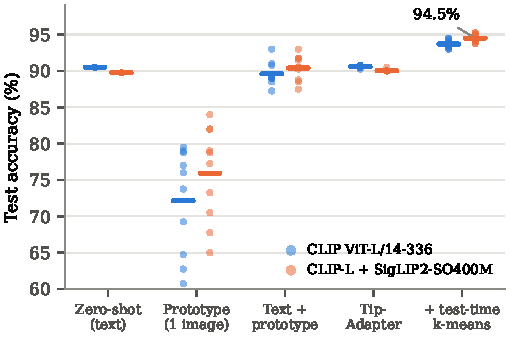
\includegraphics[width=\linewidth]{accuracy_seeds.pdf}
\vspace{-14pt}
\caption{\small Test accuracy per method. Each dot is one random one-shot split; bars are means.}
\label{fig:seeds}
\end{minipage}\hfill
\begin{minipage}[b]{0.53\linewidth}
\centering\small
\setlength{\tabcolsep}{4pt}
\begin{tabular}{lc}
\toprule
Final model, one change at a time & Accuracy (\%) \\
\midrule
Default ($\kappa{=}2$, weight 1, 20 iter., center+flip) & \textbf{94.50}\,$\pm$\,0.56 \\
$\kappa = 1$ \;/\; $\kappa = 4$ & 93.78 \;/\; 94.58 \\
image weight 0.5 \;/\; 2 & 93.20 \;/\; 95.22$^\dagger$ \\
5 \;/\; 50 iterations & 94.50 \;/\; 94.50 \\
center view only \;/\; + squashed view & 94.38 \;/\; 94.40 \\
+ unlabeled \texttt{test2} in adaptation & 94.17 \\
+ $k$-NN label propagation & 93.58 \\
\bottomrule
\end{tabular}
\captionof{table}{\small Sensitivity of the final model (means over 10 splits). $^\dagger$Chosen by test accuracy, so not reported as our score.}
\label{tab:sens}
\end{minipage}
\vspace{-8pt}
\end{figure}

\textbf{The class name is worth more than the one image.}
Zero-shot prompts alone reach 87--90.5\%, while the single-image prototype reaches only 72--80\%, and it swings by almost 20 points depending on which image is drawn (Fig.~\ref{fig:seeds}).
One photo of a kitchen or a coast can be atypical; the language model has seen thousands.

\textbf{Naive fusion barely helps.} Adding the prototype to the text scores helps backbones with weaker prompts (DFN5B +2.4) but slightly hurts CLIP-L (90.5$\to$89.6).
Tip-Adapter with its published defaults ($\alpha{=}1,\beta{=}5.5$) stays within 0.5 points of zero-shot, because its cache term is small next to $100\cdot\cos$ text logits.

\textbf{Test-time adaptation gives the real gain.} Soft $k$-means on the unlabeled test images adds 3.2--5.4 points over zero-shot for \emph{every} backbone.
It also cuts the variance across one-shot draws from $\pm$1.6 to $\pm$0.6 for the final model, because the clusters, not the single image, now define each class.
For seed 0, \emph{InsideCity} rises from 16\% to 60\% and \emph{TallBuilding} from 84\% to 96\%.
The remaining errors are genuinely ambiguous scenes: \emph{OpenCountry}$\to$\emph{Mountain} (9 of 25), \emph{InsideCity}$\to$\emph{Street} (5), and \emph{Forest}$\to$\emph{Mountain} (3).
Adding label propagation on a $k$-NN graph, or pooling the 400 unlabeled \texttt{test2} images into the adaptation, did not help (Table~\ref{tab:sens}).

\textbf{Bigger is not better here.} The three largest models, EVA02-E (5.0B parameters), OpenCLIP bigG (2.5B) and PE-Core bigG (2.4B), rank \emph{last} after adaptation, while the smallest, CLIP-L (0.43B), is the best single model.
These small grayscale scene photos are far from the web-scale color images that the newest models are tuned for.
An ensemble of two complementary models (94.50\%) beats all eight together (93.65\%).

\textbf{Robustness.} Changing any one hyperparameter or the test-time views keeps the final accuracy within 93.2--95.2\% (Table~\ref{tab:sens}).
A larger image weight (2) gives 95.22\,$\pm$\,0.84\%, but it was found by looking at test labels, so it is not our reported score.

\section{Conclusion}
With one labeled image per class, the most effective recipe was to \emph{not train} the network: keep strong vision--language encoders frozen, let carefully written prompts carry most of the class knowledge, use the single image only as an anchor, and adapt to the unlabeled test distribution at inference time.
This reaches 94.00\% (94.50\,$\pm$\,0.56\% over random draws), compared with 89.75\% zero-shot and about 76\% from the single image alone.
The key takeaways on balancing model complexity, data and compute are:
\begin{itemize}
\item \textbf{Data.} One labeled image is a noisy, high-variance signal. Combining it with the class name and the unlabeled test images matters more than any classifier trained on it.
\item \textbf{Model complexity.} Models with 2.4--5.0B parameters did not beat the 0.43B CLIP-L on this out-of-distribution grayscale data. Two complementary models (1.6B parameters in total) were both more accurate and cheaper than all eight together.
\item \textbf{Compute.} The final system needs no gradient updates. Encoding is one forward pass per image (embeddings for all 8 backbones took about 20 minutes on 8 GPUs), and the adaptation runs in under a second on a CPU, so the whole pipeline is easy to reproduce and to apply to a new folder of images.
\end{itemize}

\end{document}
